\documentclass[ ]{article}
\usepackage{pythonhighlight}
\usepackage[margin=0.5in]{geometry}
\usepackage{color, colortbl}
\usepackage{xcolor}
\usepackage{graphicx}
\usepackage{caption}



\definecolor{Gray}{gray}{0.9}
\definecolor{DarkGray}{gray}{0.5}
\definecolor{LightCyan}{rgb}{0.88,1,1}
\definecolor{yellow}{rgb}{1,1,0}

\begin{document}

\noindent
{\LARGE \textbf{Partie Appliquée}}
\vspace{5 mm}

\noindent
Dans cette section, nous allons tester et comparer les différents algorithmes de Kmeans, Kmeans++ et Kmeans++ semi-supervisées sur un jeu de données clients. Nos mesures de performances sont le coût tel qu'estimé par la fonction potentiel, ainsi que la durée d'exécution de l'algorithme.

\vspace{10 mm}

\noindent
{\Large \textbf{La Base de Données}}
\vspace{5 mm}

\noindent
La base de données contient 60366 observations (clients) et 39 variables quantitatives et qualitatives. Tous les clients sont anonymisés se qui limitera l'interprétation de l'analyse.

\noindent
Nous commençons par analyser la base de données. Ci-dessous, nous affichons la statistique d'une partie de nos données. 
\begin{center}

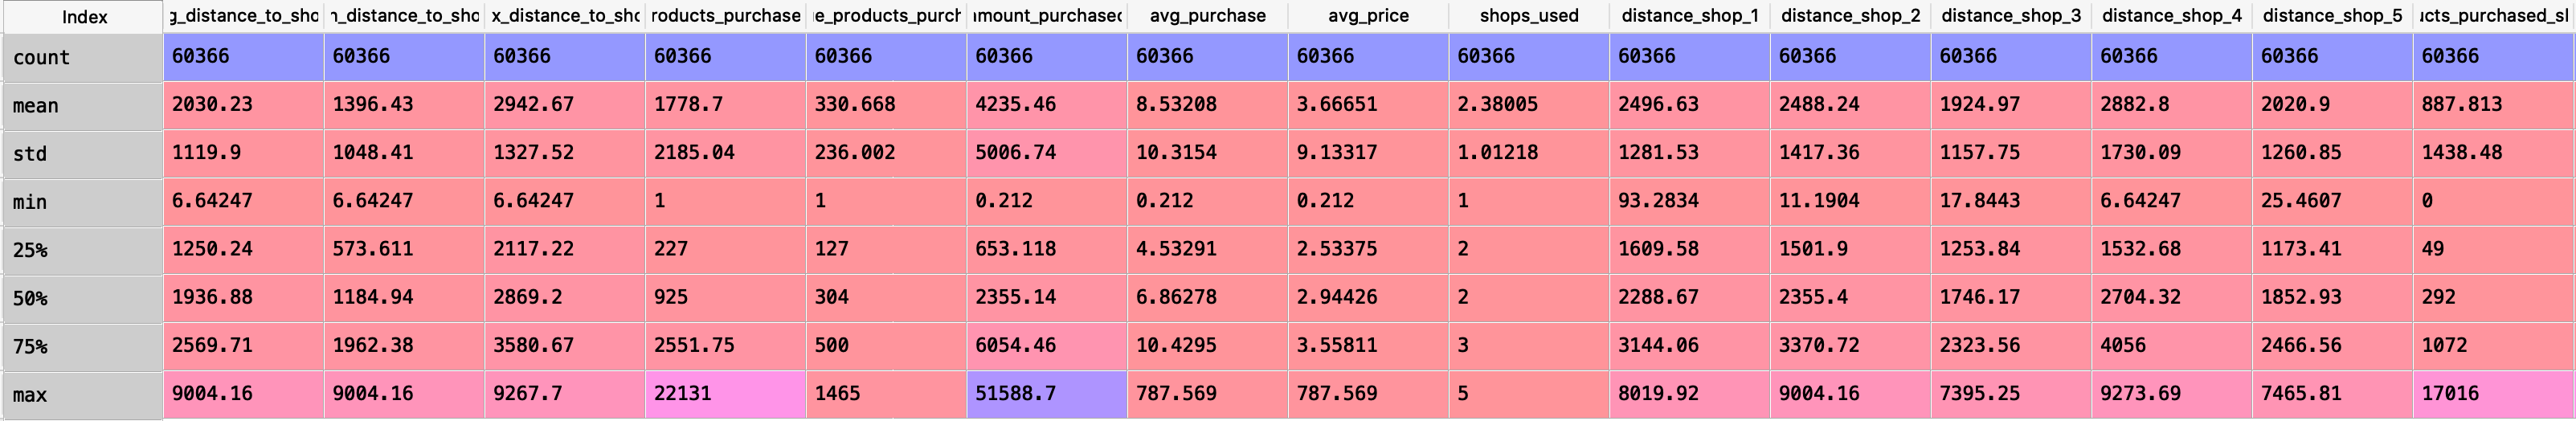
\includegraphics[scale=0.30]{summary.png}
\end{center}

\noindent
Nous voyons qu'il existe une seule variable qualitative, la variable 'shops used', les autres étant toutes des variables quantitatives continues. Nous remarquons aussi que toutes les variables quantitatives affichent de grandes dispersions. Par exemple, en regardant le nombre de produits achetés, nous voyons que certains clients achètent très peu, soit 1 seul article, tandis que d'autres achètent jusqu'à 22 131 articles, la moyenne étant 2 552.75. Ce type d'observation nous permettra de mieux interpréter les clusters proposés par les différentes versions des k-means.

\noindent
Une Analyse en Composantes Principales est implémentée afin de mieux regrouper et comprendre les variables quantitatives. Les 3 premières composantes principales expliquent moins de la moitié de l'inertie, soit 41.58\% de la variance.  Nous n'étudierons pas les résultats de l'ACP dans notre situation si ce n'est pour nous aider à trouver les composantes principales nous affichant les segmentations des clusters proposés par la méthode de kmeans.

\begin{center}
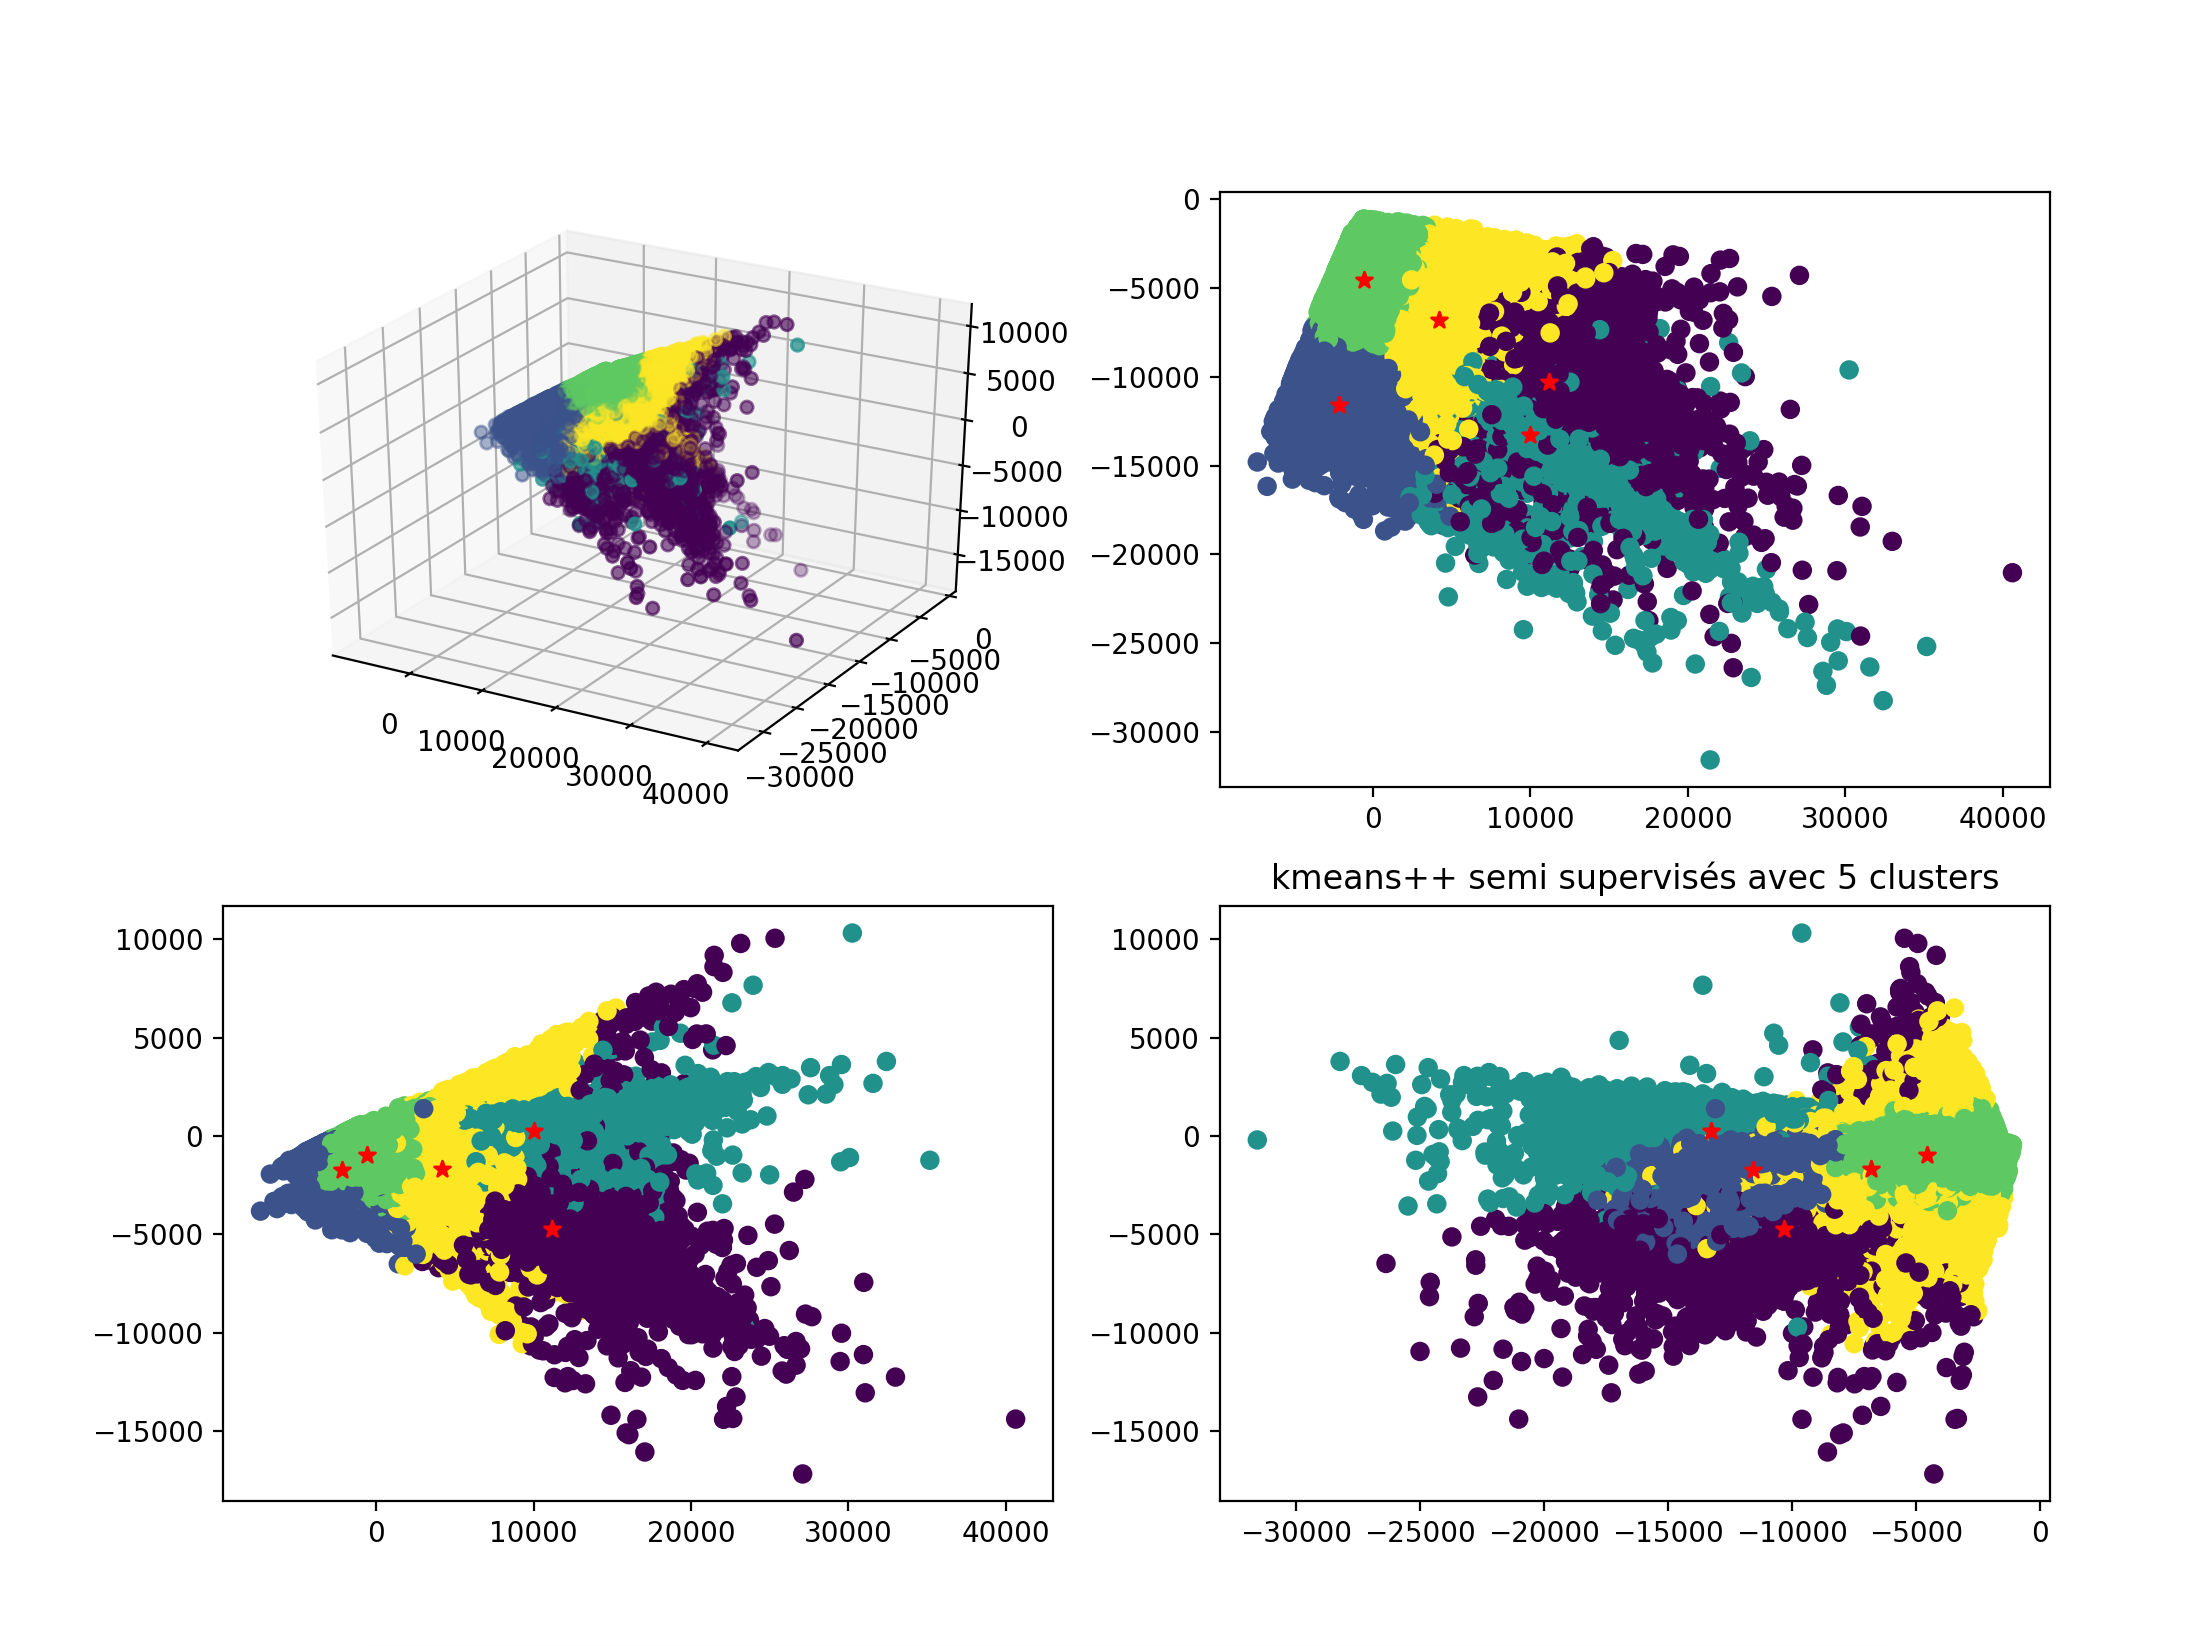
\includegraphics[scale=0.35]{ACP_3D.png}
\end{center}


\vspace{30 mm}
\noindent
\begin{large}
\textbf{Choix du nombre de clusters}
\end{large}
\vspace{5 mm}

\noindent
La méthode K-means est une méthode d'apprentissage non-supervisée. Lors de son application les données sont séparées en plusieurs classes prédéterminés de façon que les individus ayant le plus de similarité. C’est ainsi qu’une des tâches clefs est de trouver le nombre approprié de classes, k. Il existe plusieurs techniques pour déterminer le nombre de classes. Nous discuterons que des cas les plus connus : 
\begin{description}
  \item 1. Méthode du pouce:
  
  Cette méthode est une méthode approximative où le nombre de classes, k est déterminé par : 
$ k \approx \sqrt{n/2}$

    \item 2. L'indice de qualité:
    
	Afin d’évaluer la qualité de la classification, les indices inertiels , soient l’inertie intra-classes et l’inertie l’inter-classes sont souvent utilisés. L’inertie intra-classes ‘mesure le degré d’homogénéité entre les objets appartenant à la même classe‘ tandis que l’inertie inter-classes ‘mesure le degré d’hétérogénéité entre les classes.’
Il existe plusieurs indices de qualité, par exemple l’indice de Dunn, l’indice de Calinski et Harabasz (CH) ou encore l’indice de Silhouette. 
Le premier calcule la distance minimale inter-classes et ainsi plus cette distance est grande, meilleur sera la classification. 

Introduit par Kauffman et Rousseew, l’indice de Silhouette nous donne une représentation visuelle de la distance entre un point d’une classe avec les points des classes voisines. Plus le coefficient ainsi calculé est proche de 1, plus la distance avec les classes voisines (inertie inter) est grande. Ceci représente le nombre de classes optimale. À l’inverse, un coefficient proche de -1 nous indique une mauvaise classification de l’observation.


		\item 3. Méthode du coude:
		
  La méthode du coude est une technique visuelle très connue. L’idée derrière cette technique est d’implémenter la méthode K-means en parcourant k valeurs. À chacune des k valeurs, la somme des erreurs au carré est calculée et est affiché sur un graphique, nous permettant à mieux visualiser les résultats. L’objectif est de choisir la valeur k (qui sera le nombre de classes) créant un effet de ‘coude’, c’est-à-dire provoquant une baisse plus conséquente, plus soudaine de la somme des erreurs au carré. Nous disons ceci en gardant en tête que la somme des erreurs aura toujours tendance à baisser, plus la valeur de k est grande. 
  
 	 \item 4. La validation croisée:
 	 
La validation croisée regarde la stabilité des classes. Les données sont séparées en au moins deux parties. La première est utilisée pour former les classes tandis que la deuxième sert de validation. Lorsque nous parlons de stabilité, nous parlons de la fréquence à laquelle des classes similaires sont formées lorsque plusieurs itérations sont effectuées. Ainsi une plus grosse fréquence de l’apparition de mêmes classes équivaut à une plus grosse stabilité de ces classes.
 	 
\end{description}

\noindent
Dans le cadre de notre étude, nous choisissons de travailler avec la méthode du coude, une méthode que nous appliquons sur la méthode de kmeans++. Cette méthode est d'ailleurs comparée avec celle de sklearn afin de déterminer l'exactitude de l'algorithme utilisé. Le graphique ci-dessous affiche la répartition des sommes des erreurs au carré à la fois pour notre méthode, dite la méthode manuelle, ainsi que la méthode proposé par sklearn. Nous voyons une baisse plus soudaine lorsque nous avons 5 clusters. Ce sera ainsi le choix du nombre de clusters utilisé lors de l'application des algorithmes de clustering.

\begin{center}
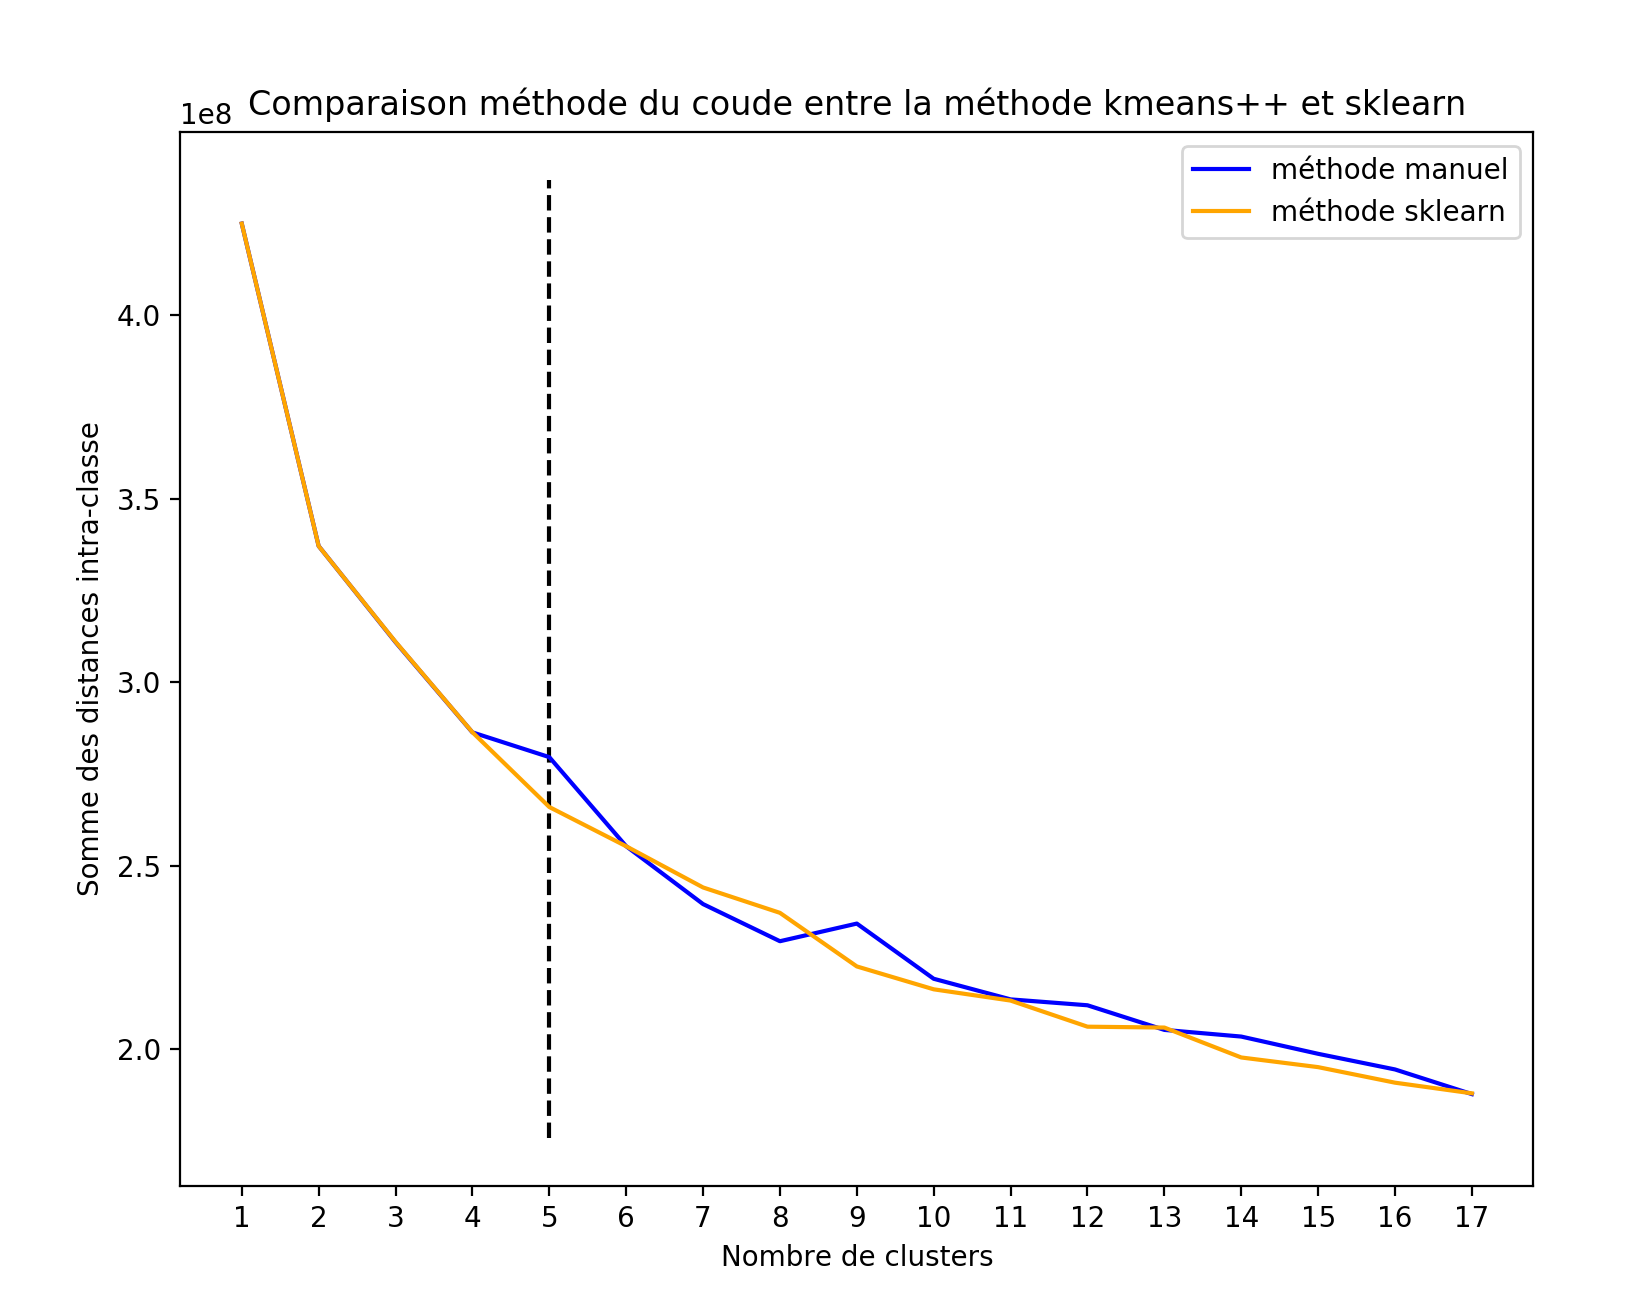
\includegraphics[scale=0.35]{Comparison_elbow2.png}
\end{center}

\vspace{10 mm}
\noindent
\begin{large}
\textbf{Observations et Résultats}
\end{large}
\vspace{10 mm}

\noindent
Dans cette section nous cherchons à présenter les résultats obtenus par les algorithmes kmeans, kmeans++ et kmeans++ semi supervisées. De plus ce dernier a été analysé plus en détails afin d'afficher l'impact des différents pourcentages de données labellisés. Comme pour l'ACP la variable qualitative a été écartée de notre analyse.
6 essaies ont été effectués afin d'évaluer le temps d'exécution des algorithmes (en secondes). La moyenne des distances intra-classes a été obtenue en se basant sur 100 simulations. Le nombre de clusters, déterminé en utilisant la méthode du coude, est 5. Nous baserons le reste de notre étude sur ces 5 clusters.

\noindent
Nous cherchons en premier lieu à comparer les résultats des différents algorithmes. Les tableaux ci-dessous les affichent.

\begin{table}[ht]
\footnotesize
\centering

\vspace{10 mm}
\caption{\textbf{Résultats en utilisant kmeans}} 

\begin{tabular}{c|c|c|c}
\hline
\rowcolor{Gray}
Temps d'exécution Minimum & Temps d'exécution Maximum & Temps d'exécution Moyen & Moyenne des distances intra-classe \\
\hline
0.867459&4.278867& 1.867284& \cellcolor{LightCyan}267024131.97\\

\end{tabular}

\centering

\vspace{10 mm}
\caption{\textbf{Résultats en utilisant kmeans++}} 

\begin{tabular}[scale=0.50]{c|c|c|c}
\hline
\rowcolor{Gray}
Temps d'exécution Minimum & Temps d'exécution Maximum & Temps d'exécution Moyen & Moyenne des distances intra-classe \\
\hline
0.952380&1.963426& 1.603216& \cellcolor{LightCyan}269311160.94\\

\end{tabular}

\centering

\vspace{10 mm}
\caption{\textbf{Résultats en utilisant kmeans++ semi-supervisées avec 60\% de données labellisées}} 

\begin{tabular}{c|c|c|c}
\hline
\rowcolor{Gray}
Temps d'exécution Minimum & Temps d'exécution Maximum & Temps d'exécution Moyen & Moyenne des distances intra-classe \\
\hline
0.386259&0.616933& 0.481936& \cellcolor{LightCyan}265971783.28\\
\end{tabular}

\end{table}

\vspace{10 mm}


\noindent 
Tel qu'attendu la durée d'exécution moyenne de l'algorithme de kmeans est plus longue que celle du kmeans++ et du kmeans++ semi-supervisée (avec 60\% de données labellisées). Cette dernière est d'ailleurs en moyenne 3 fois plus rapide que le kmeans ou le kmeans++. Au niveau du coût de la fonction nous voyons que le kmeans ++ semi supervisée affiche à nouveau le meilleur résultat (avec la plus petite distance moyenne intra-classes sur 100 simulations). Nous notons toutefois que la distance intra-classe moyenne lorsque kmeans est utilisé est plus petite que celle du kmeans++.  Bien qu'il soit préférable que ce soit l'inverse, cette observation peut être dû au fait que le jeu de données en question ne soit pas adapté pour les kmeans. 


\vspace{10mm}
\noindent

\begin{table}[ht]
\footnotesize
\centering

\caption{\textbf{Résultats en utilisant kmeans++ semi-supervisées avec 25\% de données labellisées}} 
\begin{tabular}{c|c|c|c}
\hline
\rowcolor{Gray}
Temps d'exécution Minimum & Temps d'exécution Maximum & Temps d'exécution Moyen & Moyenne des distances intra-classe \\
\hline
0.534357&0.759242& 0.629477& \cellcolor{LightCyan}265972507.4\\

\end{tabular}

\centering

\vspace{10 mm}
\caption{\textbf{Résultats en utilisant kmeans++ semi-supervisées avec 99\% de données labellisées}} 

\begin{tabular}{c|c|c|c}
\hline
\rowcolor{Gray}
Temps d'exécution Minimum & Temps d'exécution Maximum & Temps d'exécution Moyen & Moyenne des distances intra-classe \\
\hline
0.115119&0.288531& 0.232994& \cellcolor{LightCyan}265976831.1\\
\end{tabular}

\end{table}

\vspace{10 mm}

Des tableaux ci-dessus, nous voyons que plus le pourcentage de données est labellisé, plus le temps d'exécution est rapide. Toutefois, nous ne pouvons pas dire autant des distances intra-classe moyenne. En effet lorsque les données sont labellisés à 99\% nous avons une inertie plus élevée que lors que les données sont moins labellisés. Une nouvelle fois la problématique pourrait venir du jeu de données, ou encore du fait que la supervision est en fait une pseudo-supervision car les données réelles n'étaient pas disponible. Ainsi cela explique la variation des inerties moyennes. C'est pour cela que nous nous baserons davantage sur la durée d'exécution comme mesure de performance.

\noindent
Nous cherchons désormais à interpréter les résultats obtenus sur le jeu de données utilisé dans cet étude. Le graphique ci-dessous affiche les 5 clusters ainsi que leurs centres, tel que proposé par l'algorithme kmeans++ semi-supervisée. 

\begin{center}
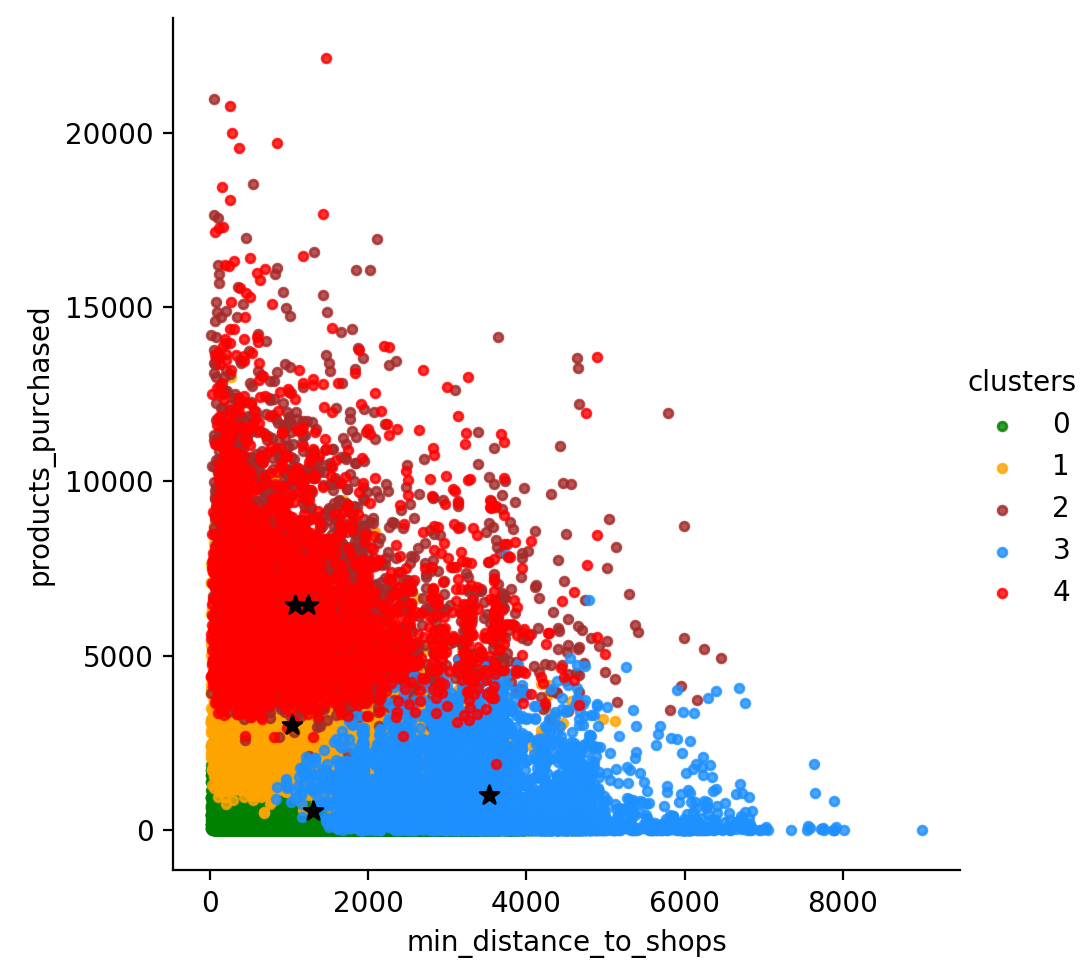
\includegraphics[scale=0.40]{kmeanspp_clusters.png}
\end{center}


\vspace{10 mm}
\noindent
Nous pouvons clairement voir que les clusters 1 et 3 (orange et rouge) sont moins distinctes entre elles contrairement aux autres clusters. Effectivement, les centres de ces deux clusters sont très proches suggérant que nous aurions pu regrouper ces deux clusters. Nous avons choisi ici de représenter le nuage de points associé aux variables \verb|products_purchased| et \verb|min_distance_to_shops|. Ces variables ont été choisies car les clusters étaient les mieux représentées lors de l'ACP.  

\noindent
Ce que nous pouvons déduire du graphique est que les clients appartenant aux clusters 4 sont ceux parcourant les plus petites distances des magasins à l'inverse de ceux du cluster 0. D'ailleurs nous voyons que ces derniers achètent le moins de produits, tout comme les clients du cluster 2. Ainsi, nous pouvons établir un lien entre la distance parcouru pour aller au magasin et le nombre de produits acheté. En général, plus un client devra parcourir une plus grosse distance, moins il ira au magasin, et le moins de produits il achetera. Sur un plan commercial et de marketing, ce seront ainsi les clients des clusters 1,3 et 4 qui devraient être ciblés comme étant des acheteurs potentiels.


\vspace{5 mm}
\noindent
Nous cherchons désormais à établir d'autres liens avec les variables utilisés dans notre jeu de données. Nous commençons par analyser la variable qualitative \verb|shops_used|. Le graphique ci-dessous nous affiche la répartition des magasins ciblés dans l'étude. Les magasins 4 et 5 sont les proches des clients. Pour le magasin 3 et le 4 (bien que celui-ci est moins distincte que le magasin 3) , il est clair que moins le client voyage, plus il achète des produits. Toutefois vu la grande quantité de données, il est difficile de bien différencier les clusters, ainsi il faudra d'autres graphiques pour confirmer nos résultats.

\begin{center}
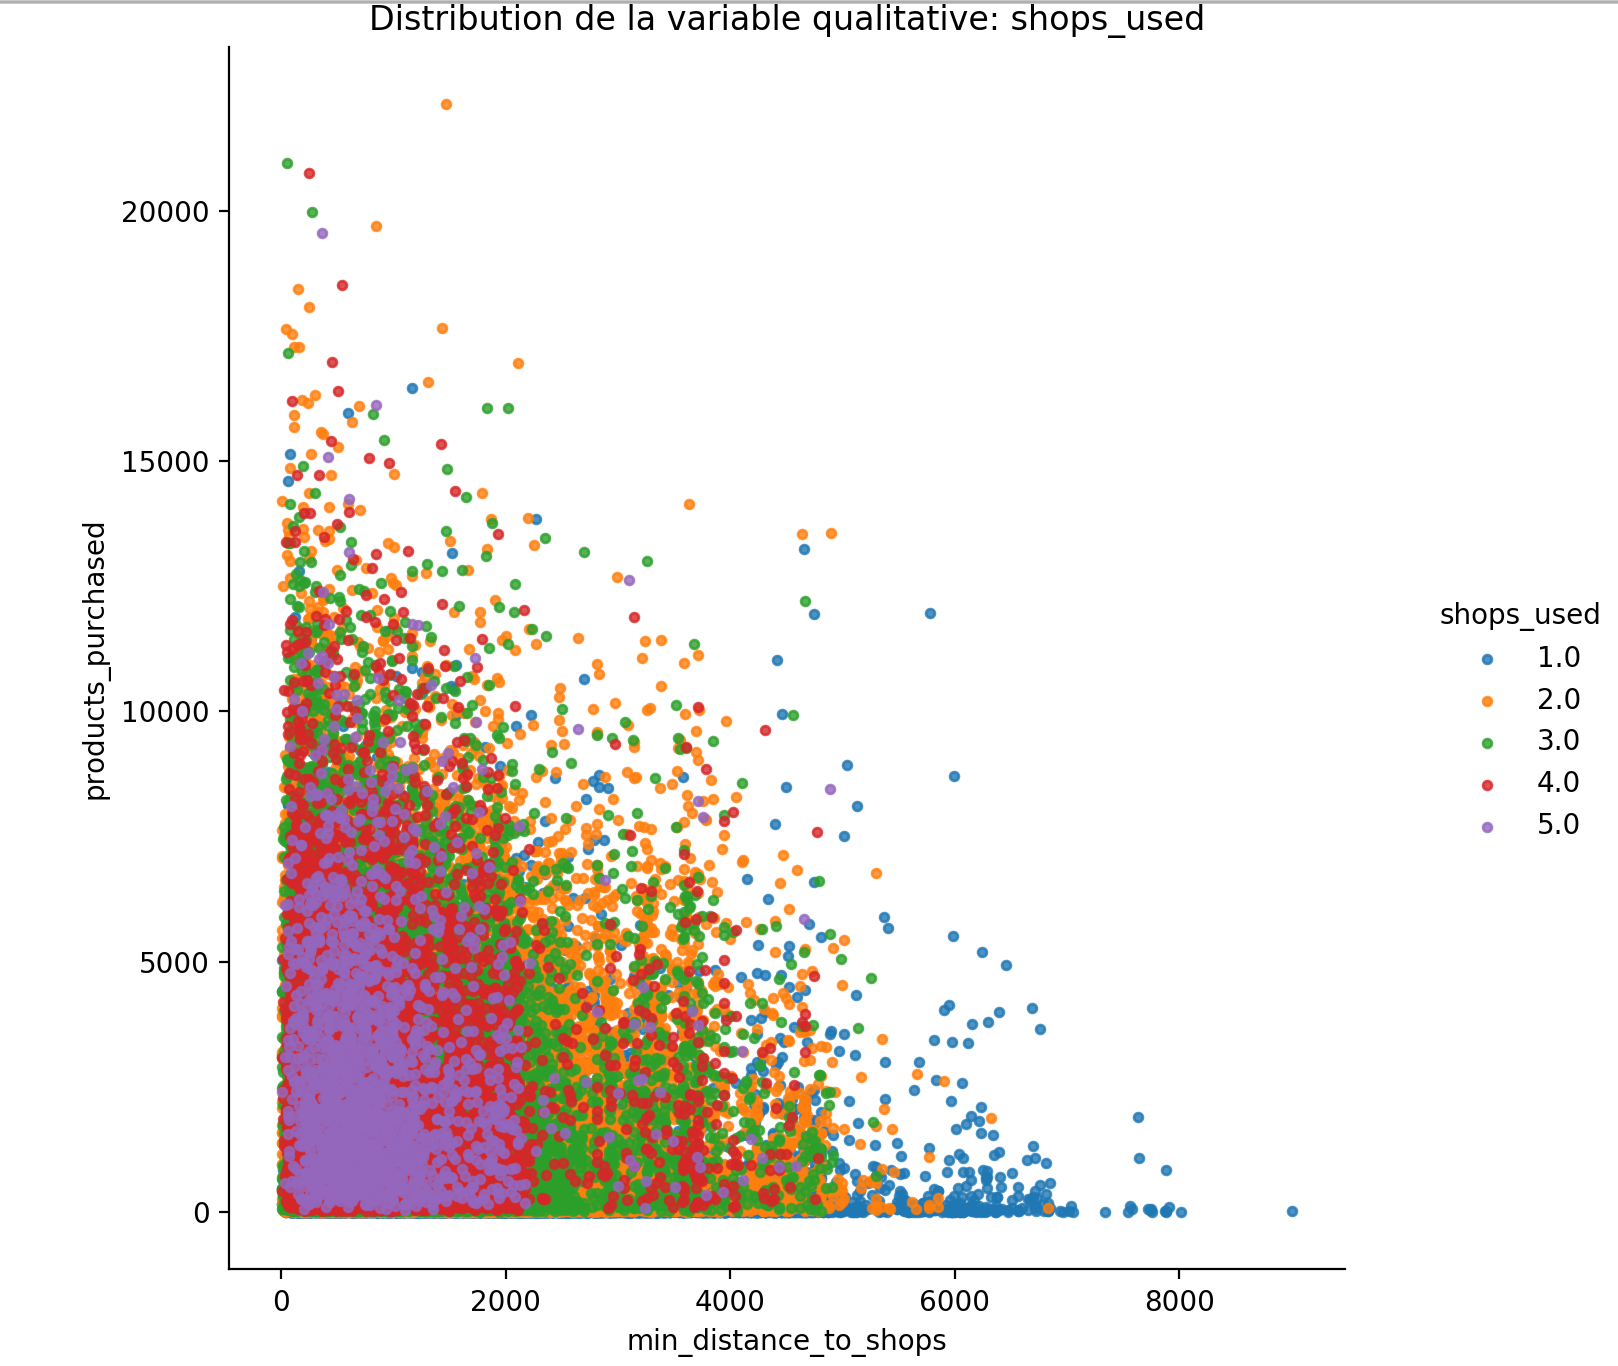
\includegraphics[scale=0.40] {shops_used.png}
\end{center}

\noindent
Les graphiques ci-dessous affichent la relation entre la distance pour aller à chaque magasin et le nombre de produit achetés dans ces magasins. Nous voyons dans le  premier graphique que les clients des clusters 1, 2 et 3 semble avoir une préférence pour le magasin 1. Les clients du cluster 5 sont ceux qui semblent habiter le plus loin du magasin 1. En revanche bien qu'ils y sont plus loin, leur consommation semble être un peu plus grande qu'au magasin 2, suggérant qu'ils préfèrent acheter les produits du magasin 1 au 2. Pour les 3 derniers graphiques, il est difficile d'établir un lien évident car les observations sont mélangés et peu distinguable. Nous nous baserons sur d'autres graphiques afin de tirer des conclusions.


\begin{center}
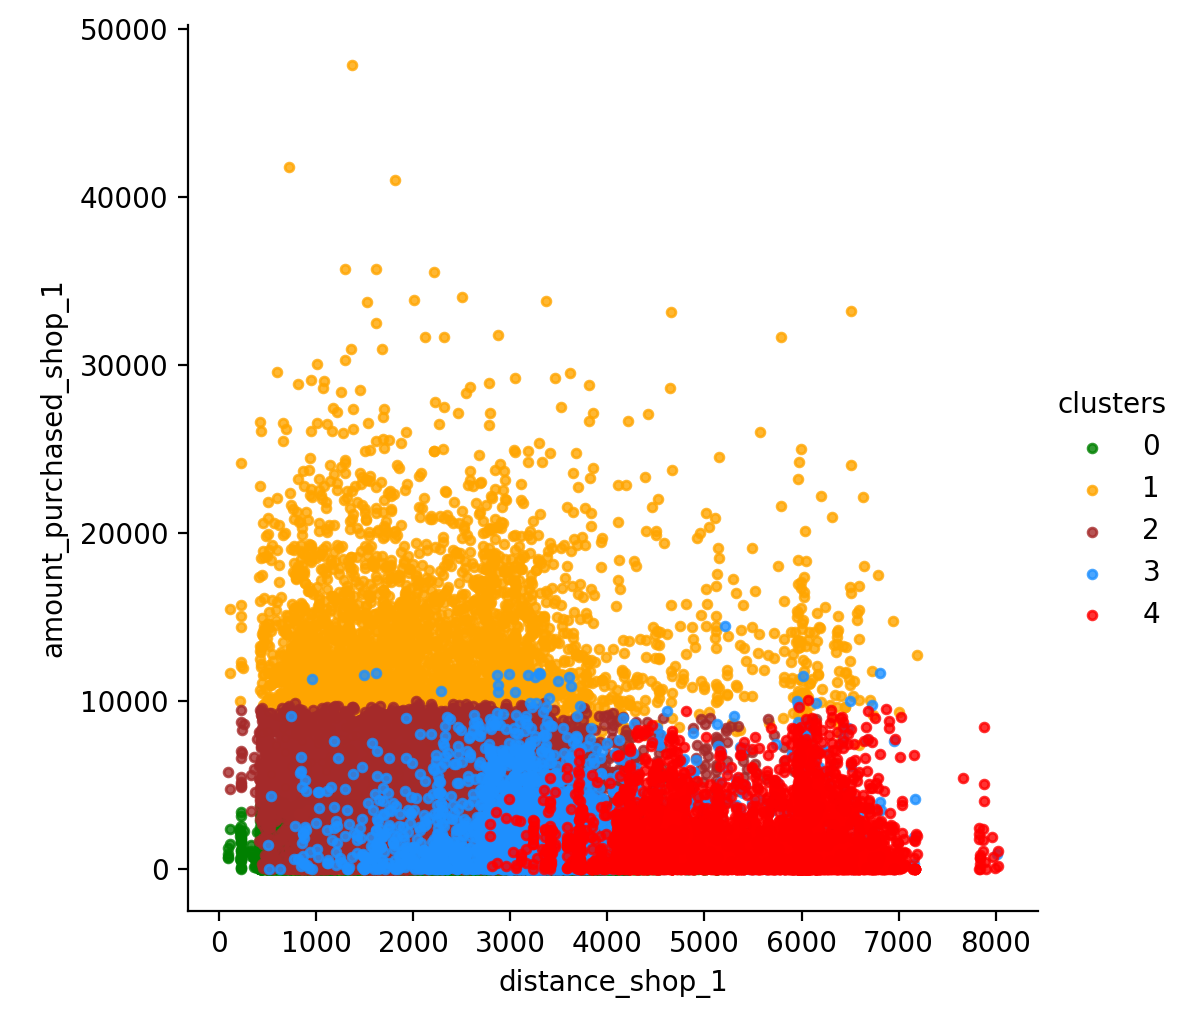
\includegraphics[scale=0.30] {shop1_amountpurchased.png}
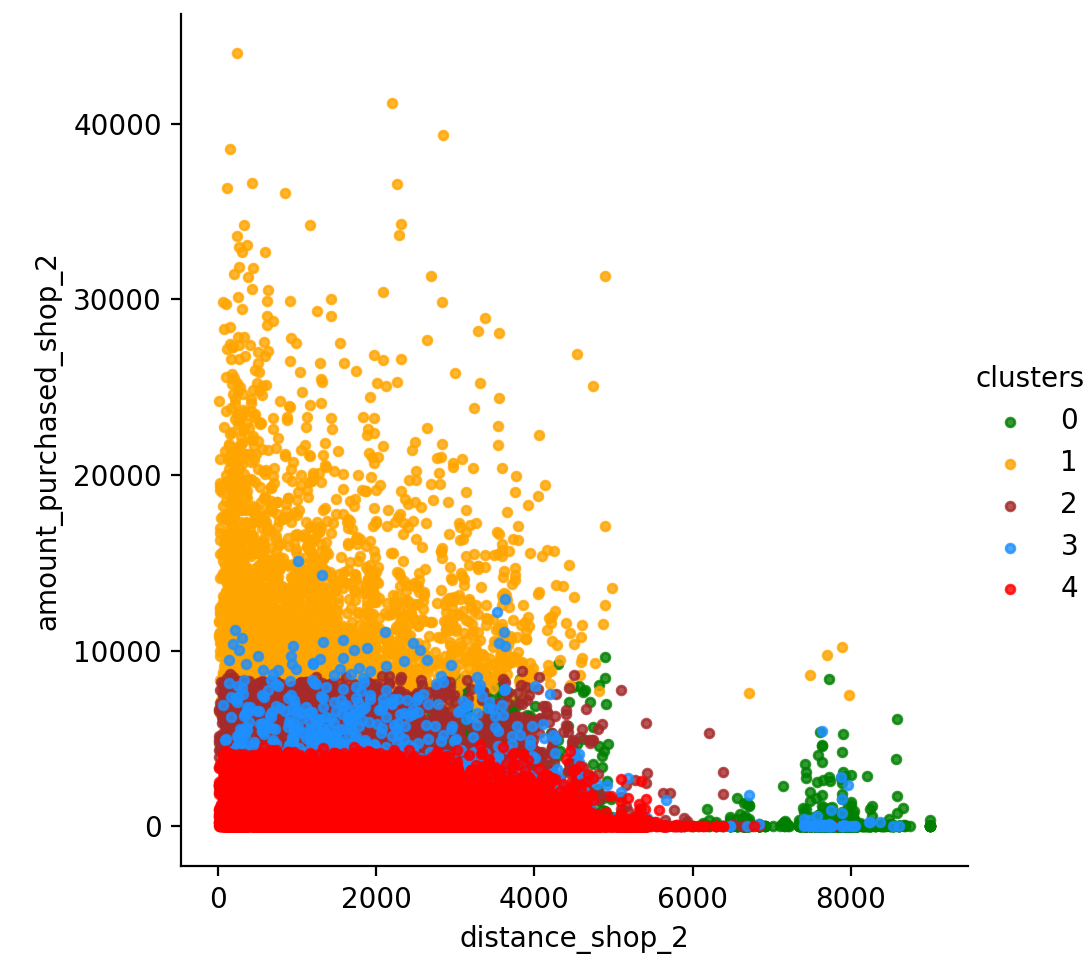
\includegraphics[scale=0.30] {shop2_amountpurchased.png}
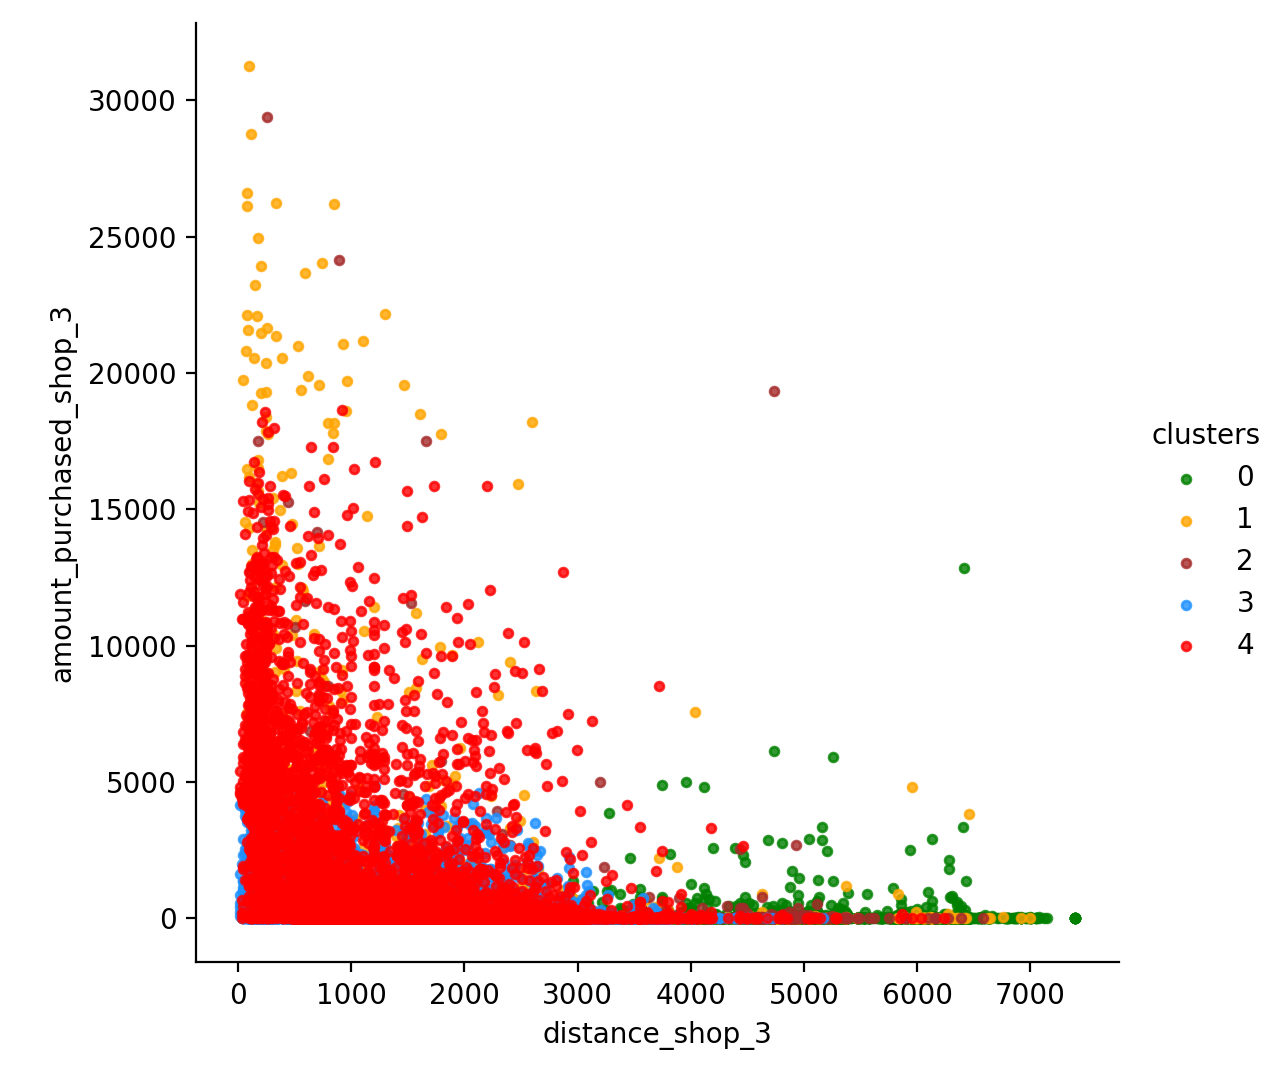
\includegraphics[scale=0.30] {shop3_amountpurchased.png}
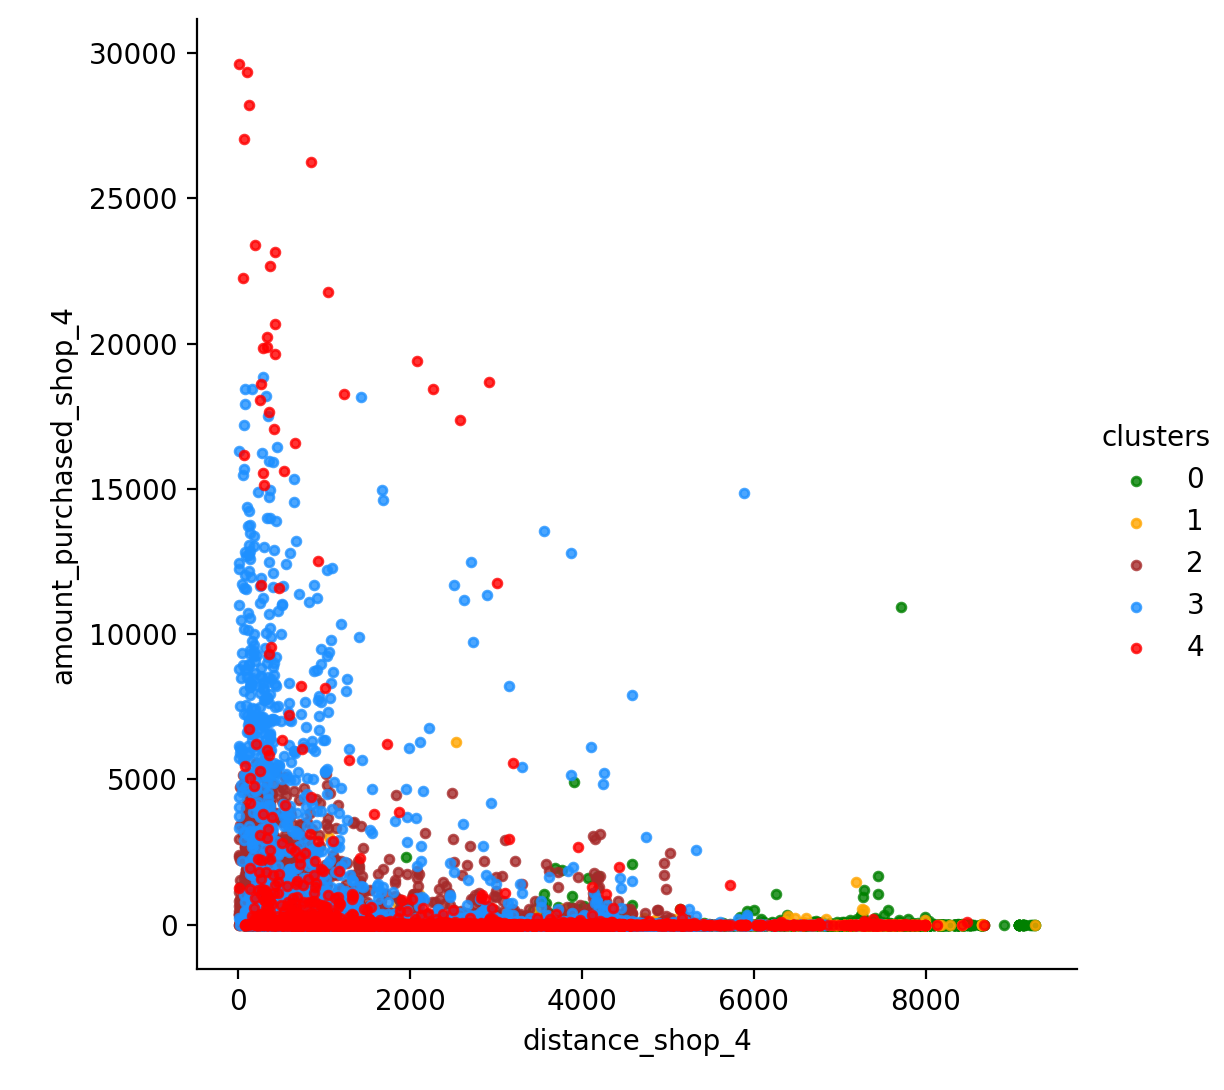
\includegraphics[scale=0.30] {shop4_amountpurchased.png}
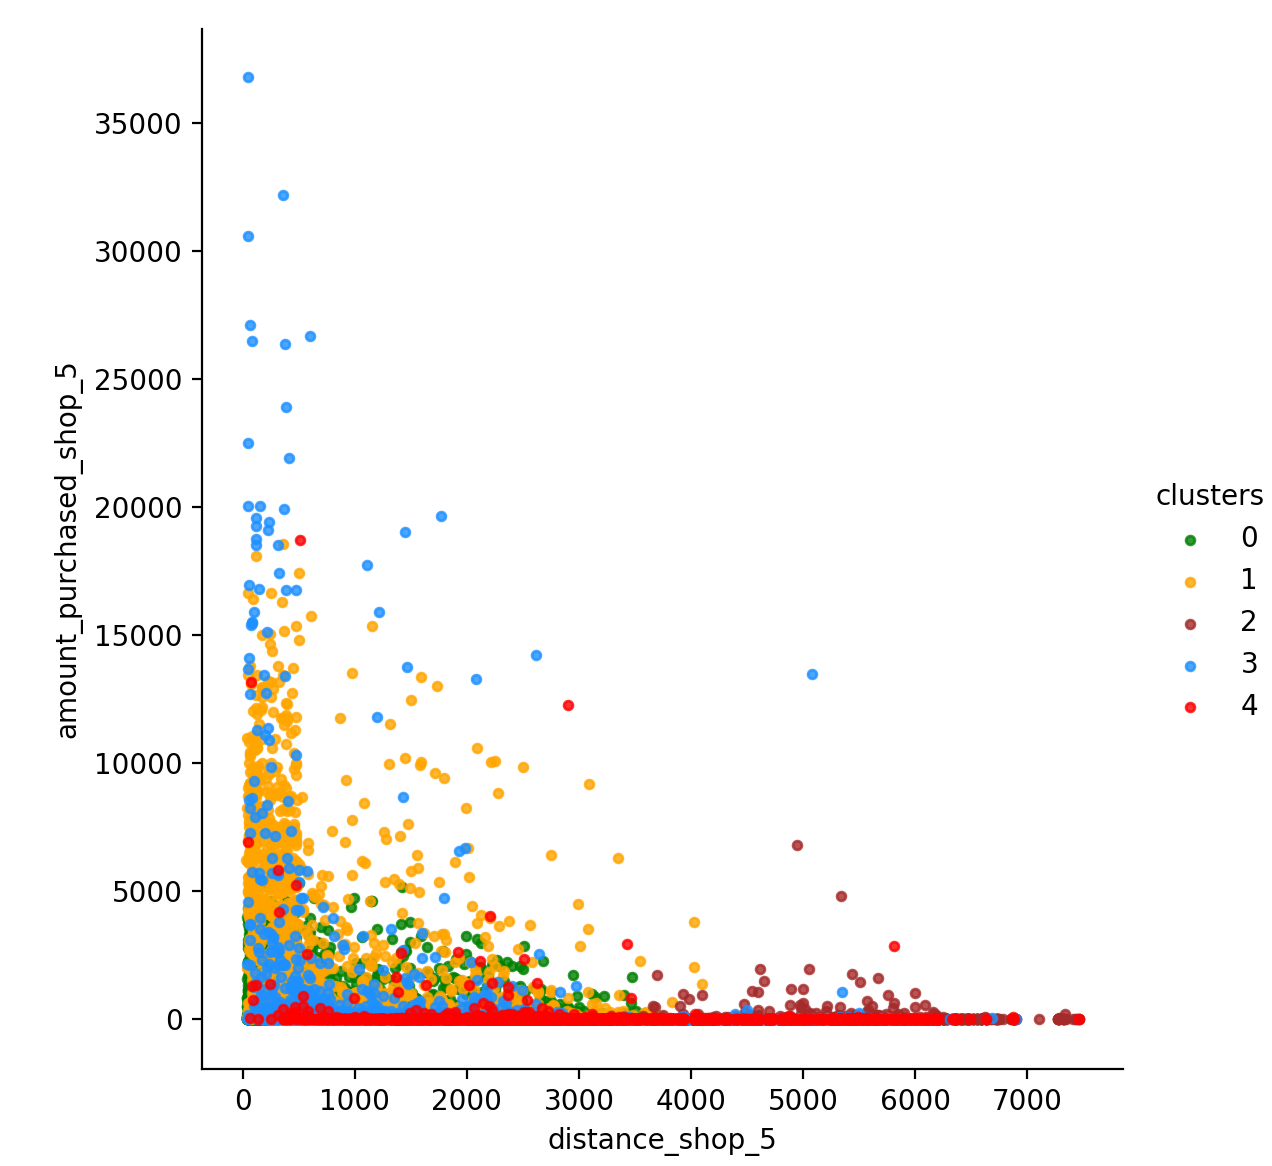
\includegraphics[scale=0.30] {shop5_amountpurchased.png}
\end{center}


Nous utilisons des diagrammes à barre (voir ci-dessous) afin de nous aider à mieux comprendre le nombre de clients allant dans les magasins ainsi que les vrai nombre de produits vendus. Nous voyons que le magasin 5 est celui qui vend le plus de produits (unique et globalement) et c'est celui qui affiche le plus petit prix moyen des produits. Ainsi, le magasin 5 et 4 sont les magasins les plus vendeurs. Le magasin est celui qui vend les produits les plus chers. Il n'est donc pas étonnant de voir qu'il vend une plus petite quantité de produits. Finalement, nous voyons quand même que plus de clients vont aux magasins 1 et 2, avec un minimum de client allant au magasin 5. De ces observations nous comprenons que les magasins 1 et 2 sont des magasins qui vendent des produits plus cher, ainsi bien que les clients puissent y aller plus souvent, ils ne vont pas nécessairement acheter les produits de ces magasins. 




\noindent
\begin{center}
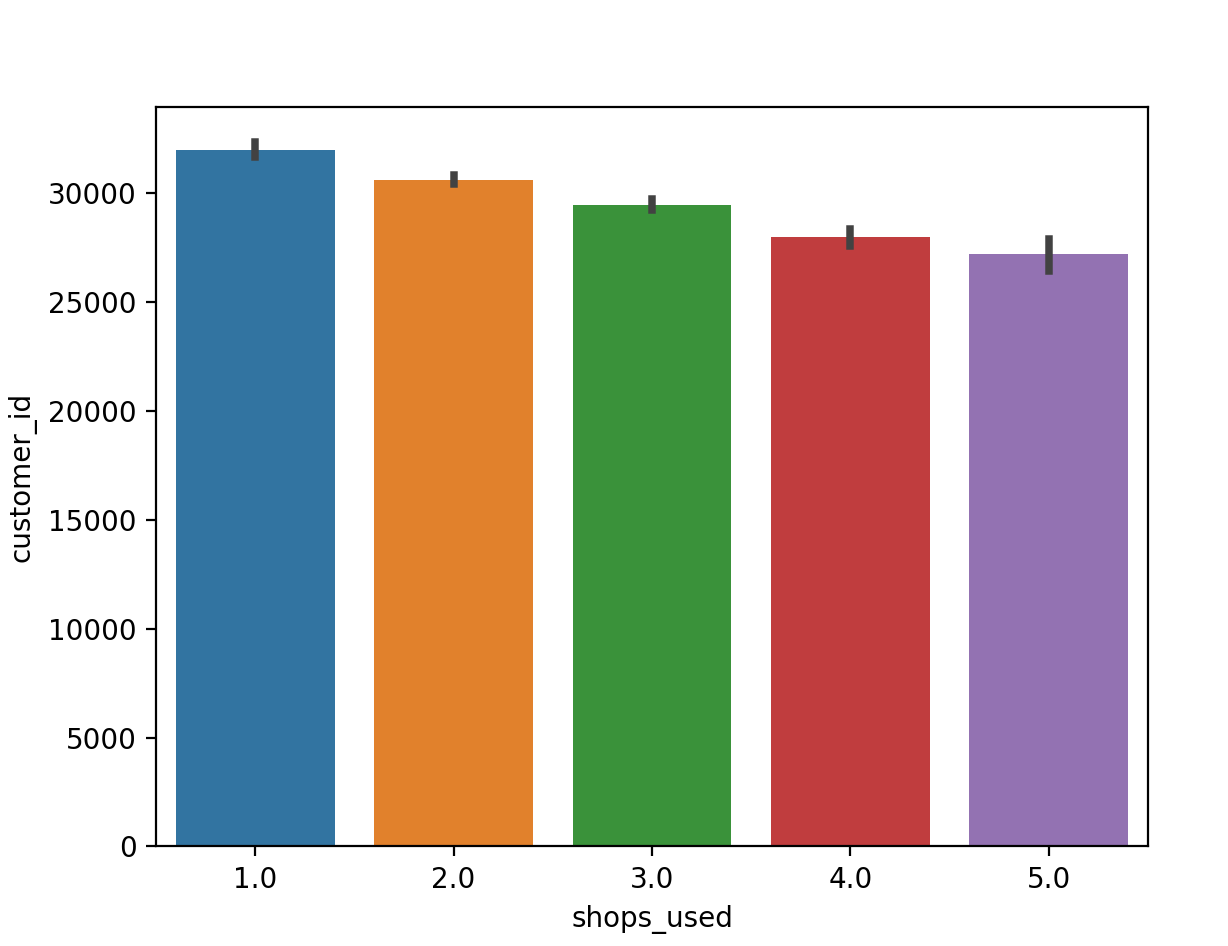
\includegraphics[scale=0.20] {clients_shops.png}
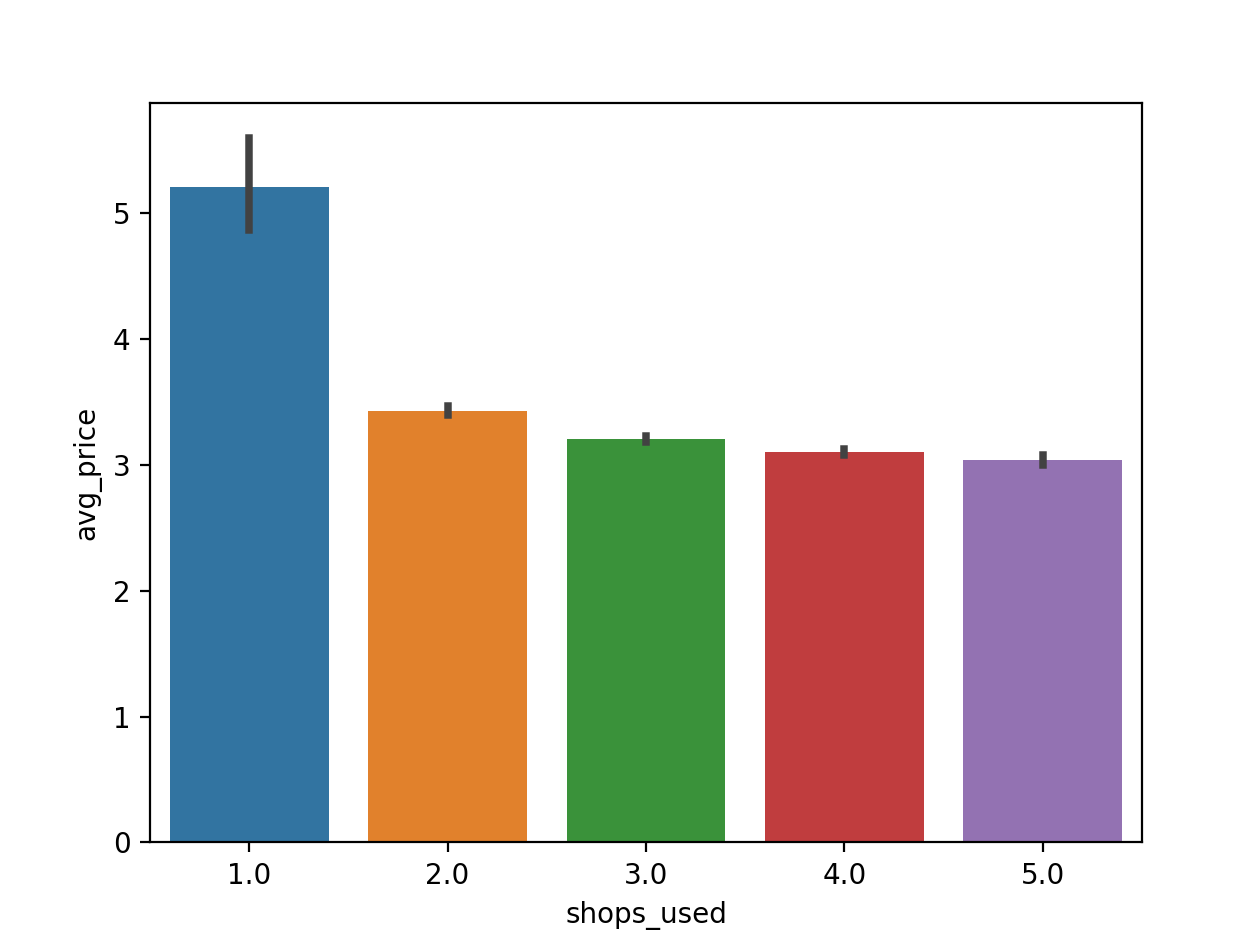
\includegraphics[scale=0.20] {price_shops.png}
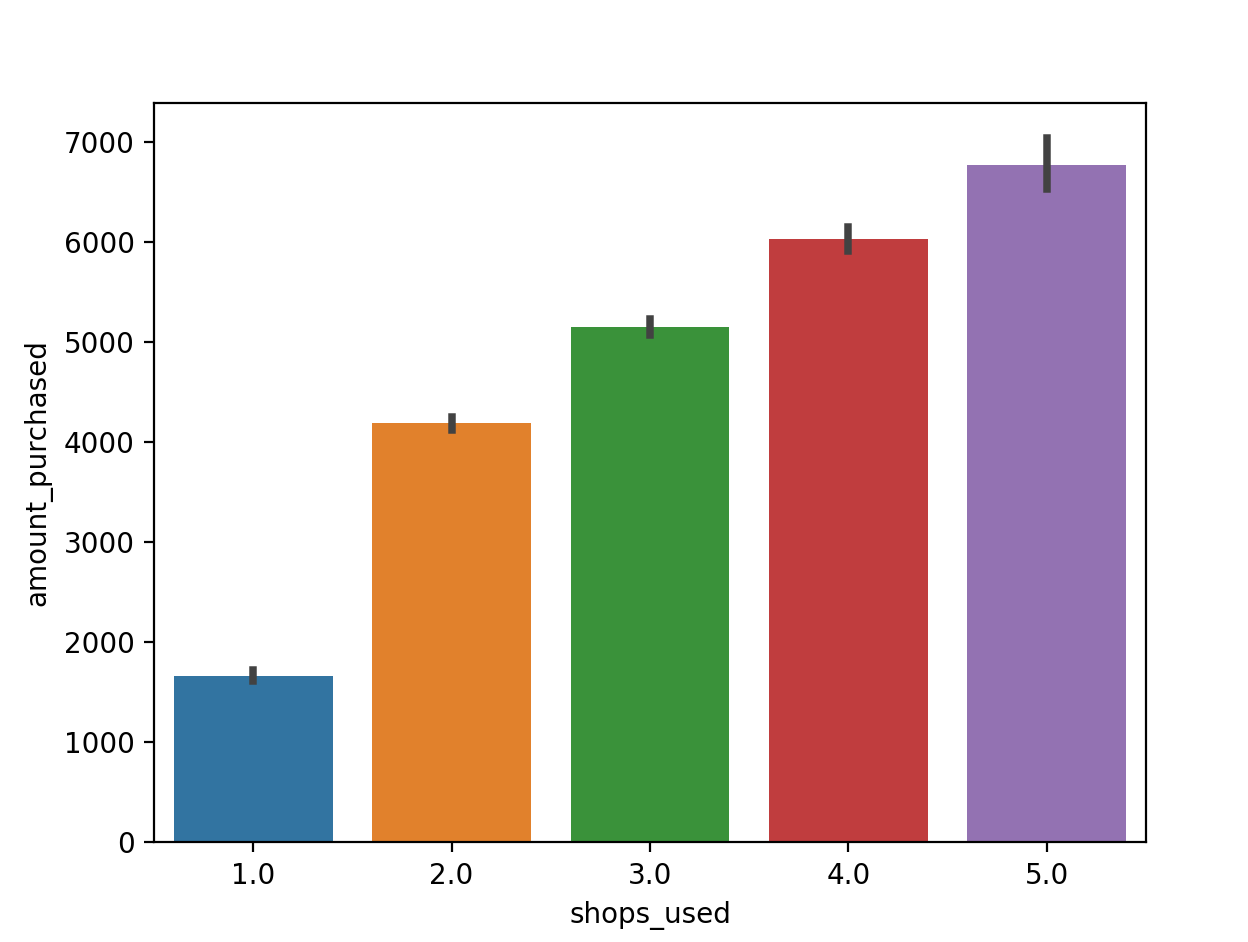
\includegraphics[scale=0.20] {amountpurchased_shops.png}
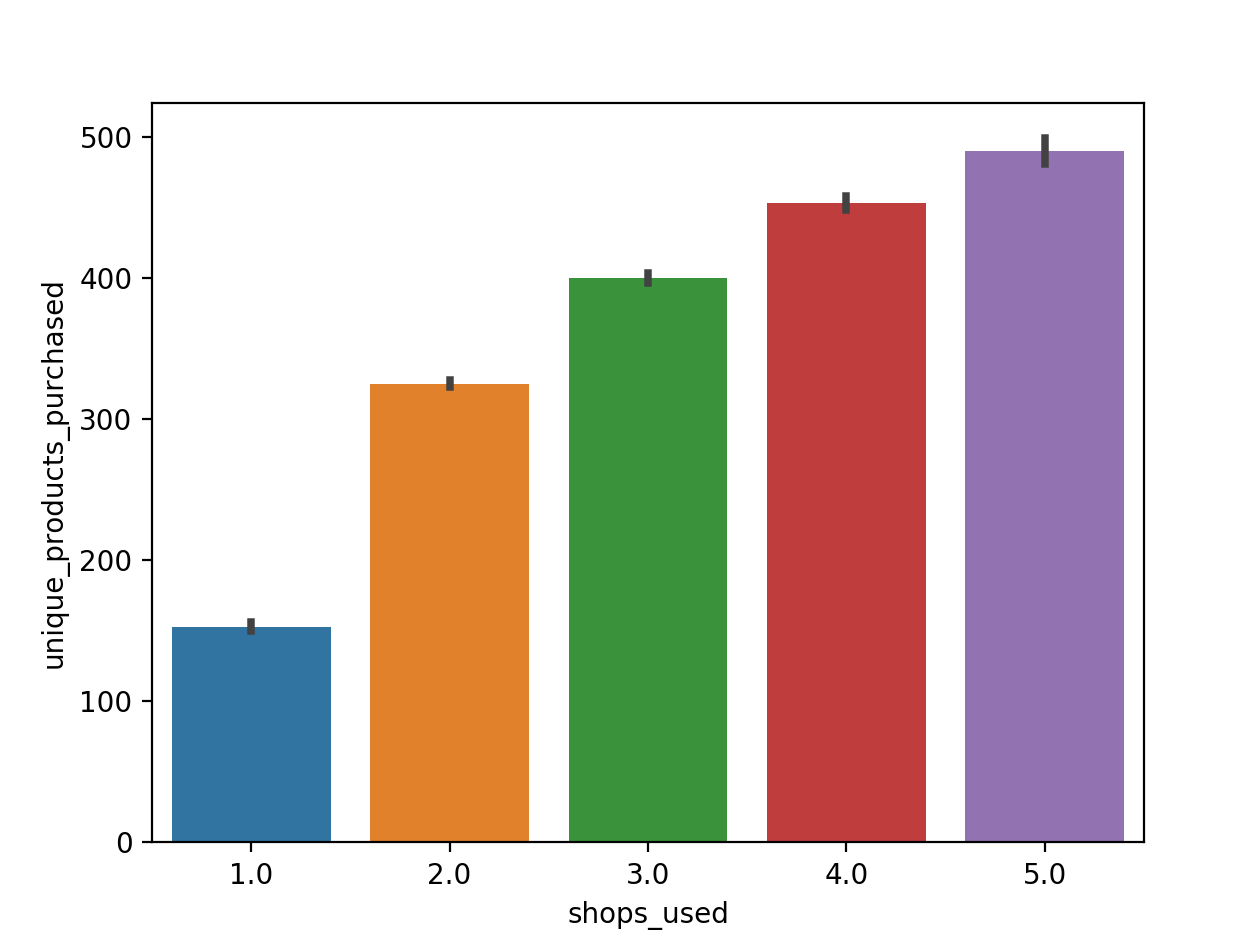
\includegraphics[scale=0.20] {unique_shops.png}
\end{center}

\noindent
Toutes les observations nous pousse à dire que la consommation diminue lorsque les prix augmentent, et ainsi les magasins les moins chers, soient 4 et 5, sont ceux vendant le plus de produits. Ils ont également plus de produits uniques que les magasins plus chers comme le 1 et 2. Ces derniers attirent beaucoup de clients, mais ceux-ci n'achèteront pas nécessairement les produits, d'où le fait que ces types de magasins vendent moins de produits. Au niveau des marges d'affaires de ces magasins, nous voyons dans le diagramme ci-dessous qu'il n'y a pas de grandes différences entre ces boutiques. Effectivement, le nombre de consommation est compensé par le prix, ce qui fait que la vente moyenne reste plus ou moins égale.

\begin{center}
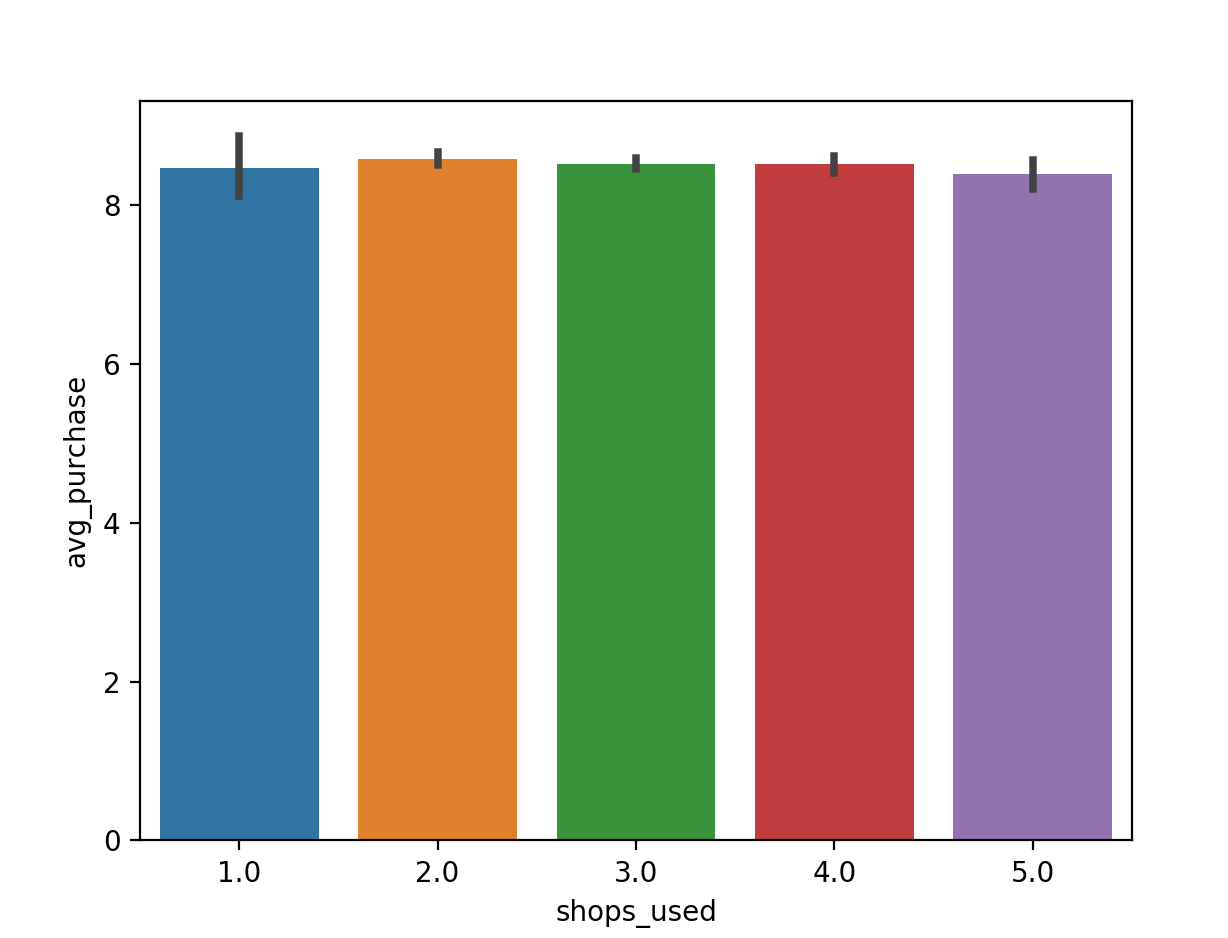
\includegraphics[scale=0.30] {avgpurchased_shops.png}
\end{center}

\noindent
Nous cherchons maintenant à lier ces observations avec les clusters obtenus par les kmeans++ semi-supervisée nous pouvons établir une tendance. Pour cela nous utilisons à nouveau des diagrammes de barres qui affichent le nombre d'individus de clusters qui achètent dans les différents magasins. À l'aide de ces graphiques (voir ci-dessous), nous pouvons établir que certains magasins attirent davantage certains clients.

\noindent
Le magasin 1 attire les individus du cluster 1, tandis que le magasin 2 attire plus le cluster 2, le magasin 3 attire les individus des clusters 1 et 2, le magasin 4 quant à lui attire les clients des clusters 2 et 3, et finalement le magasin 5 attire principalement les individus du cluster 4 et 3. Dans tous les cas le cluster 0 est celui qui est le moins représenté, confirmant le fait que ce cluster pourrait facilement être regroupé avec un autre cluster. 

\noindent
Ainsi dans cet étude la segmentation des clients peut être faite en se basant sur les magasins.

\begin{center}
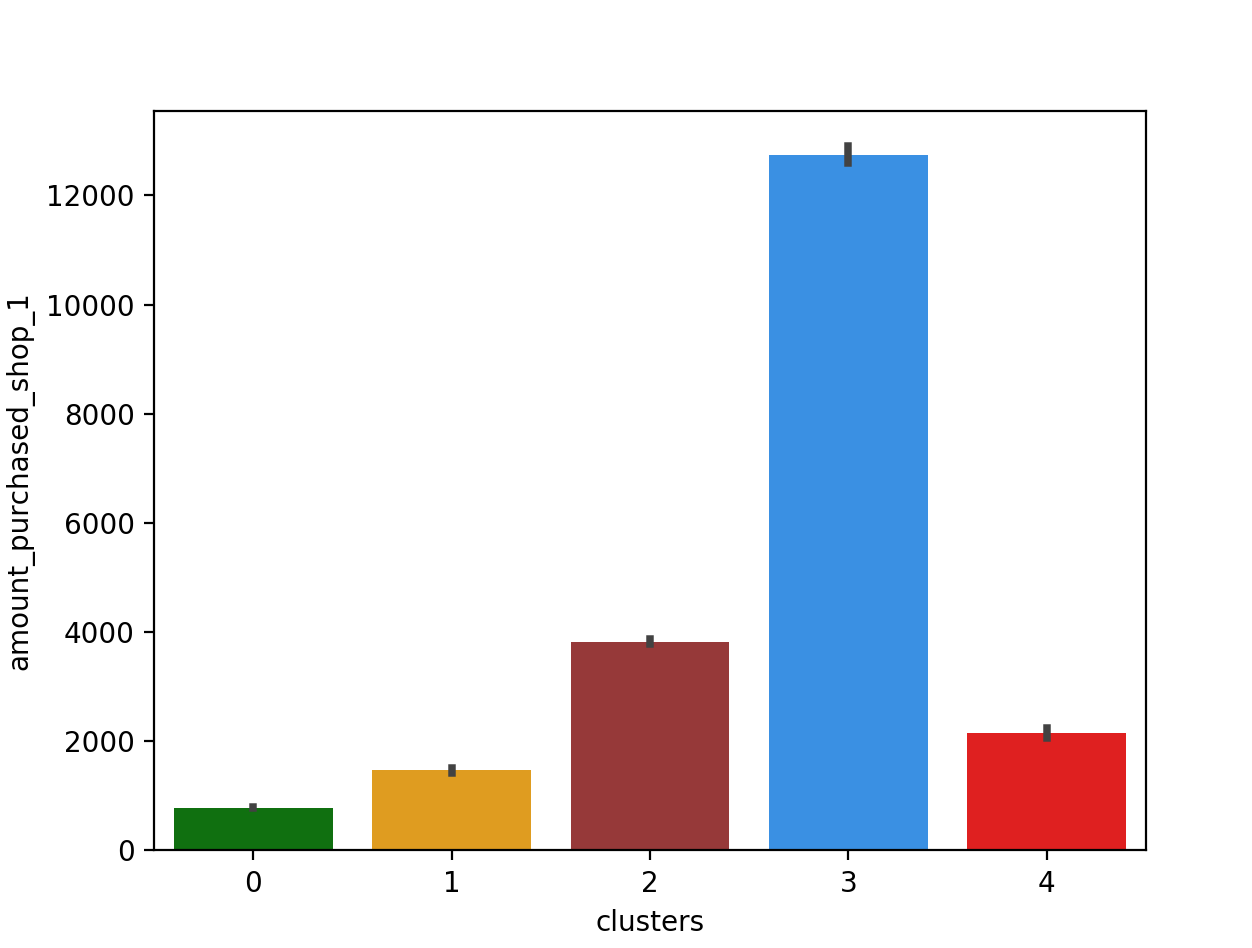
\includegraphics[scale=0.20] {cluster_shop1.png}
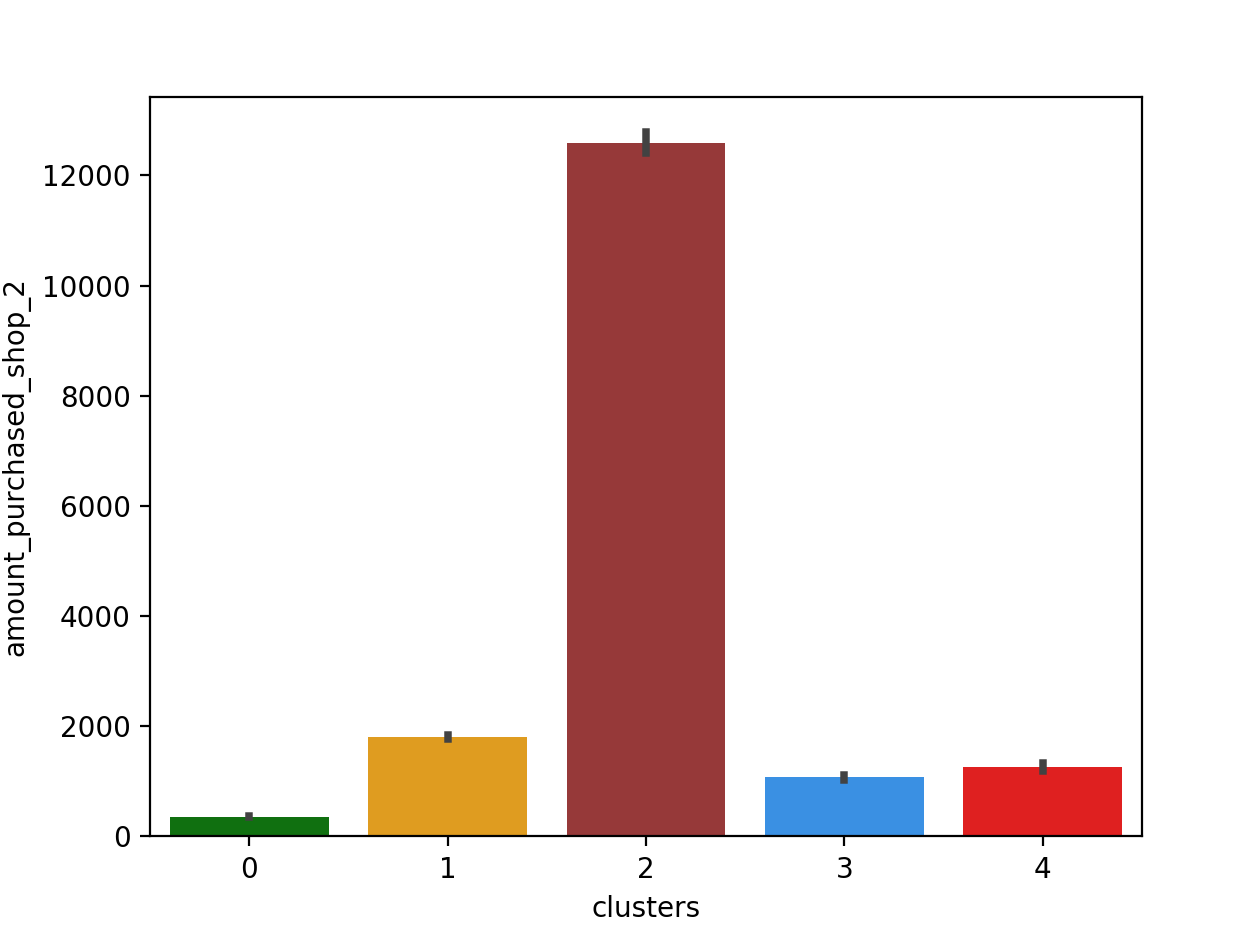
\includegraphics[scale=0.20] {cluster_shop2.png}
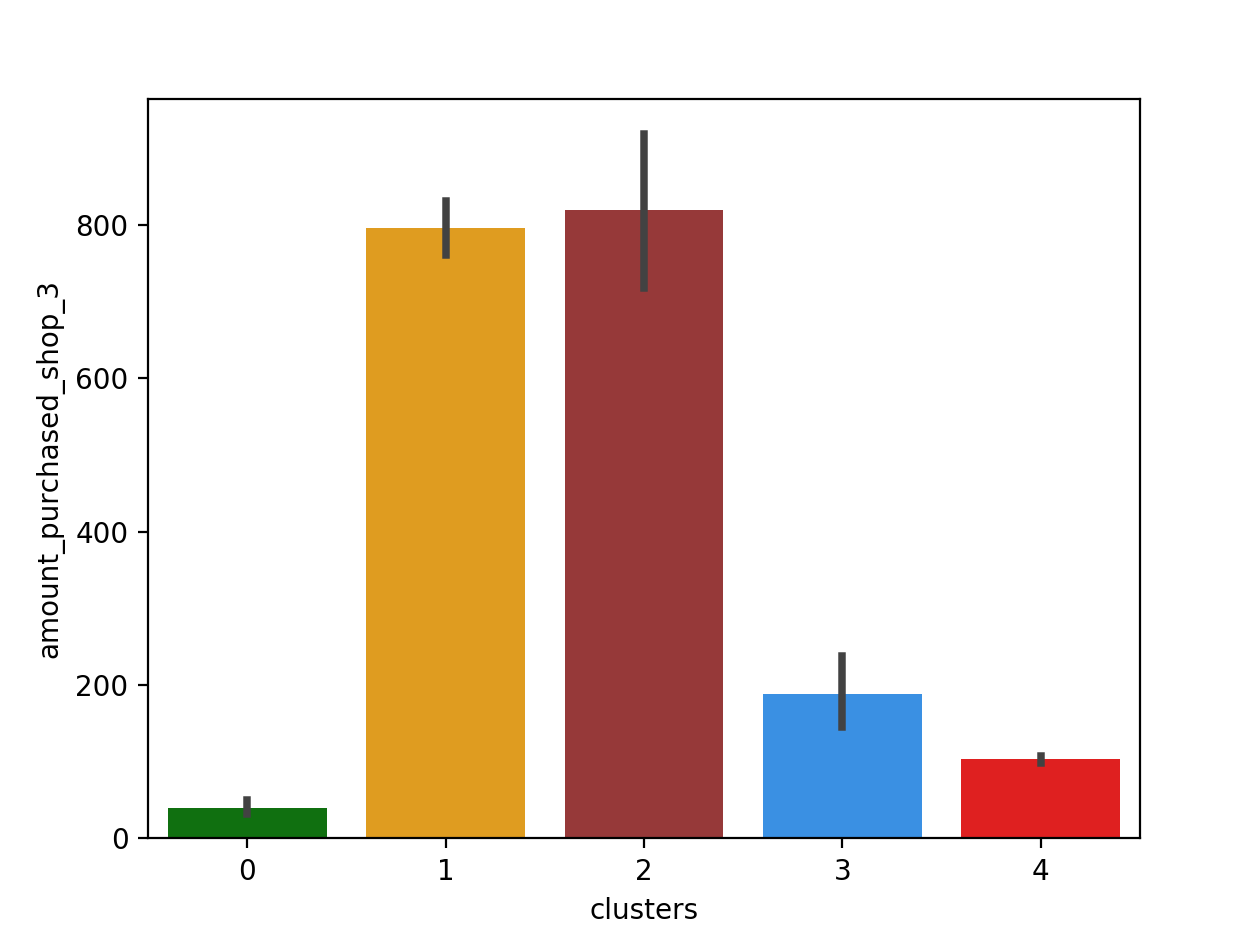
\includegraphics[scale=0.20] {cluster_shop3.png}
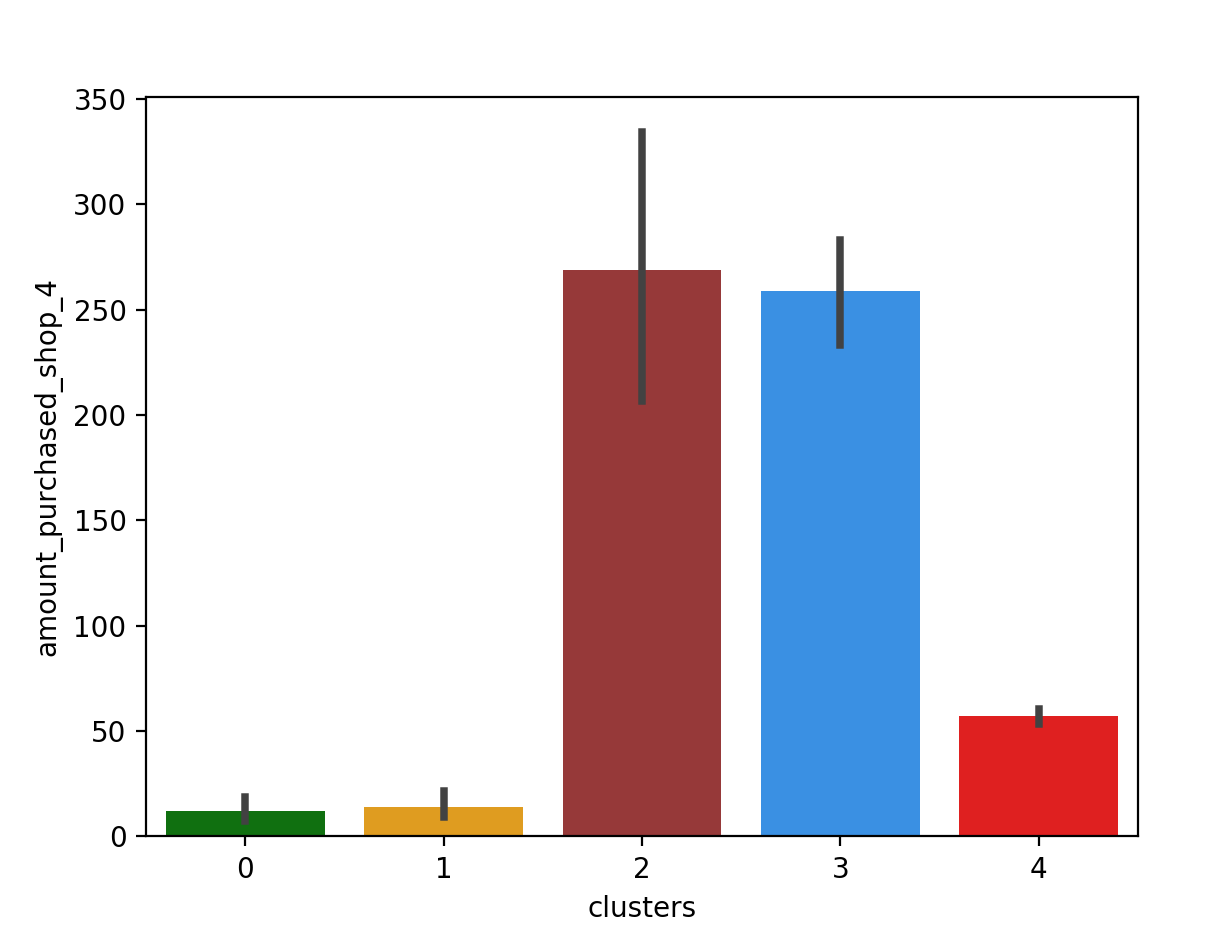
\includegraphics[scale=0.20] {cluster_shop4.png}
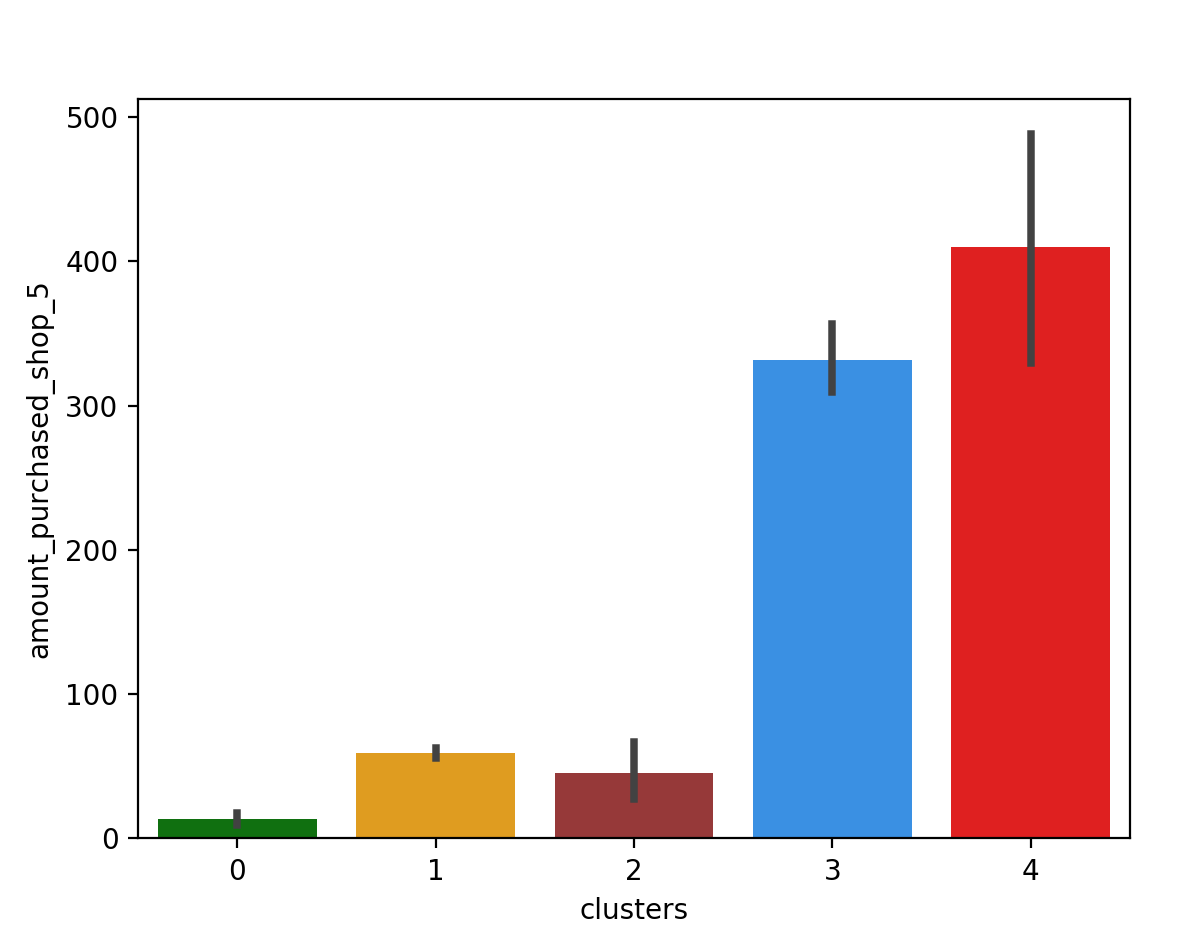
\includegraphics[scale=0.20] {cluster_shop5.png}
\end{center}

\vspace{10 mm}





\end{document}
